\chapter{Currents of Electricity}
\begin{itemize}
    \item The \emph{number density} \(n\) is defined as the number of particles per unit volume.
    \item The \emph{drift velocity} \(v\) is the \emph{average} velocity at which \emph{charge carriers} move through a \emph{conductor} when there is \emph{electric current in the conductor}.
    \item Deriving the equation \(I=nAvq\):
    \begin{enumerate}
        \item Assume that the \emph{current is constant}. Then, \(I=\frac{Q}{t}\).
        \hspace*{0pt}\hfill \(\highlight[yellow]{[n]}\)
        \item Assume that there are \(N\) charge carriers passing through a cross-sectional area \(A\) in time \(t\), and that \emph{each} of them carries an \emph{identical amount of charge} \(q\). Then, the \emph{total charge} that passing through \(A\) in time \(t\) is
        \[Q=Nq \tag*{\(\highlight[yellow]{[N,A(t),Q(t)]}\)}.\]
        \item Assume that the \emph{number density} \(n\) of charge carriers is \emph{uniform}, and let \(V\) be the volume covered by the current in time \(t\). Thus,
        \[N=nV \tag*{\(\highlight[yellow]{[n,V(t)]}\)}.\]
        \item Furthermore, since the current travels at some velocity \(v\),
        \[V=A\Delta x=Avt \tag*{\(\highlight[yellow]{[v]}\)}.\]
        \item Therefore, 
        \[I=\frac{Q}{t}=\frac{Nq}{t}=\frac{nVq}{t}=\frac{nAvtq}{t}=nAvq.\]
    \end{enumerate}
    \item Elementary charge \(e=1.6\times 10^{-19}C\) (Charge of an electron/proton).
    \item The \emph{potential difference} between \emph{two points} of a circuit is defined as the amount of electrical energy \emph{converted} to other forms of energy \emph{per unit charge} moved \emph{between} the two points. 
    \item \emph{Ohm's Law} states that the \emph{current} flowing in a \emph{conductor} is \emph{directly proportional} to the \emph{potential difference across it} under \emph{constant physical conditions}.
    \item \emph{Resistance} is defined as the \emph{ratio} of the \emph{potential difference across} the conductor to the \emph{current} flowing through it.
    \item \emph{Resistivity} \(\rho\) is the \emph{proportionality constant} between the \emph{dimensions of a specimen of a material} and its \emph{resistance} such that 
    \[R=\frac{\rho L}{A}.\]
    \newpage
    \item Electrical Components
    \begin{longtable}{|Sc|Sc|Sc|}
        \hline
        Types of Conductors & Changes to Resistance & Reason\\
        \hline
        \begin{minipage}{0.25\textwidth}
            Metallic conductor at constant temperature
        \end{minipage} &  
        \begin{minipage}{0.3\textwidth}
            \begin{itemize}
                \item At \emph{ constant temperature} this is an Ohmic conductor.
                \item Has \emph{constant resistance}. Ratios of \(V/I\) is constant.
            \end{itemize} 
            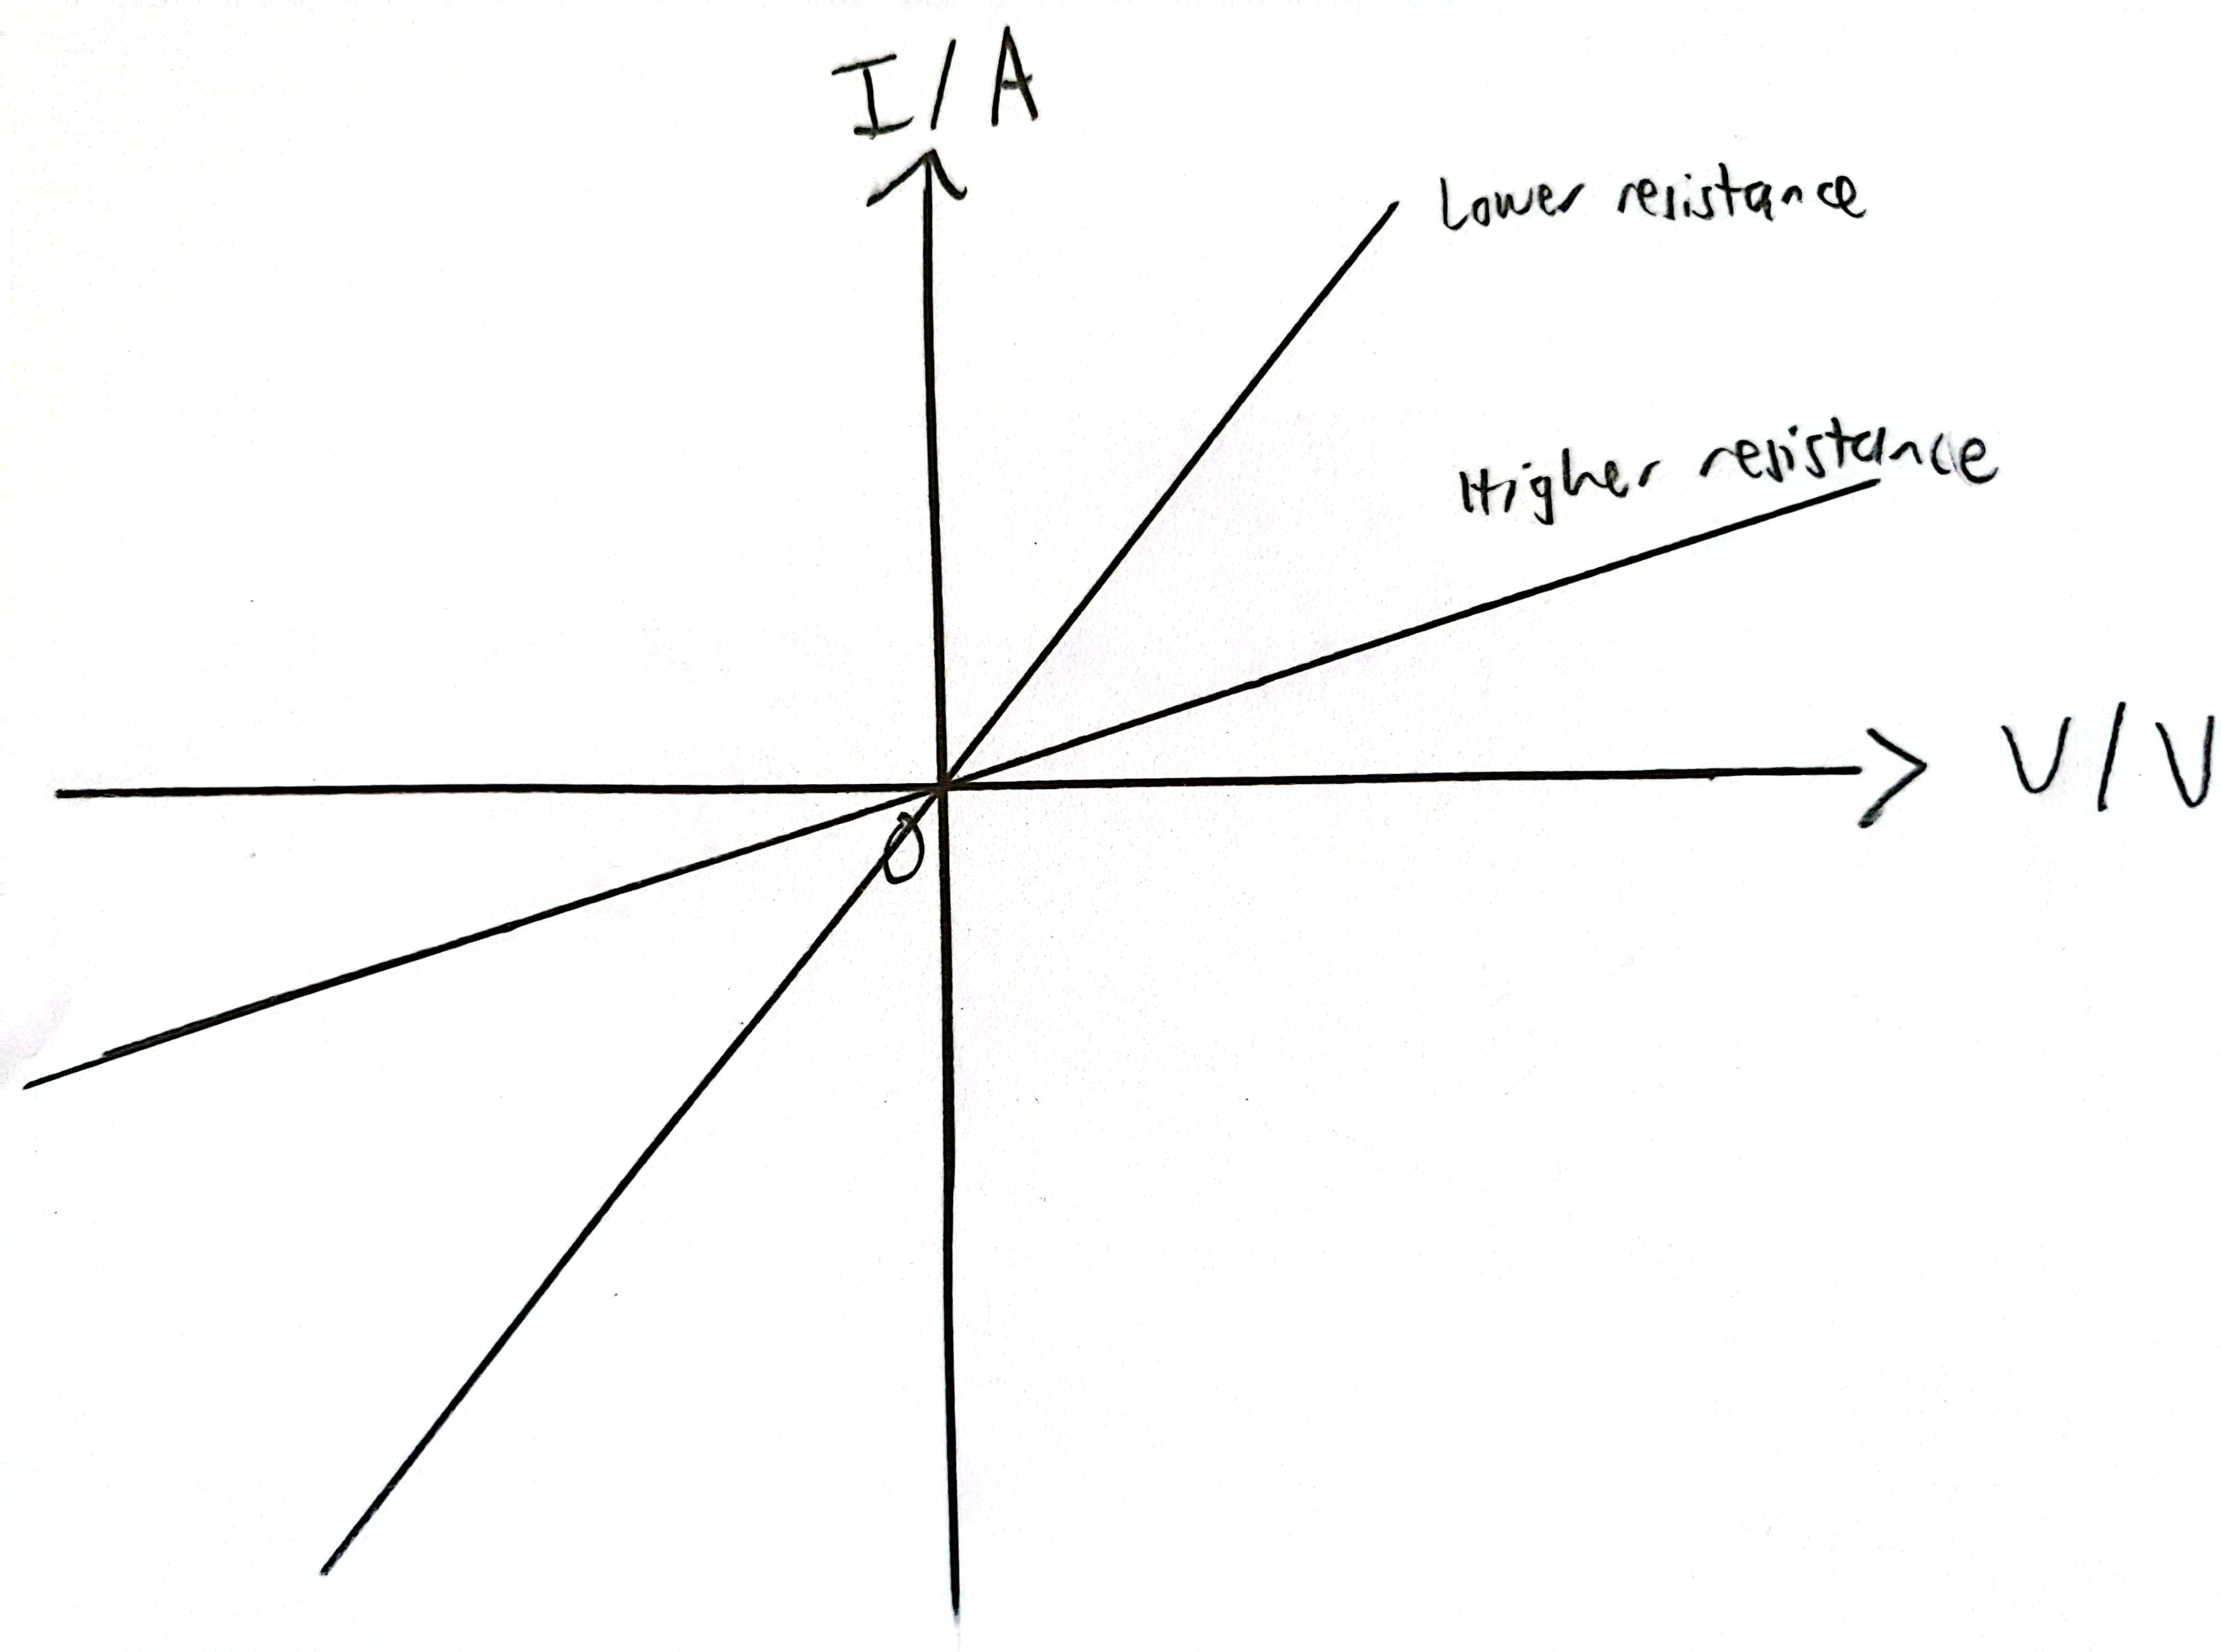
\includegraphics[width=\textwidth]{../images/MetallicConductor I-V.jpg}
        \end{minipage} &
        \begin{minipage}{0.3\textwidth}
            \begin{itemize}
                \item At \emph{constant temperature}, the \emph{number of free electrons} and the \emph{rate of atomic vibration} is constant.
                \item A resistor at a different constant temperature will have a difference resistance, and hence, \(V/I\) ratio. 
            \end{itemize}
        \end{minipage}\\
        \hline
        \begin{minipage}{0.25\textwidth}
            Semiconductor Diode\\[5mm]
            \begin{center}
                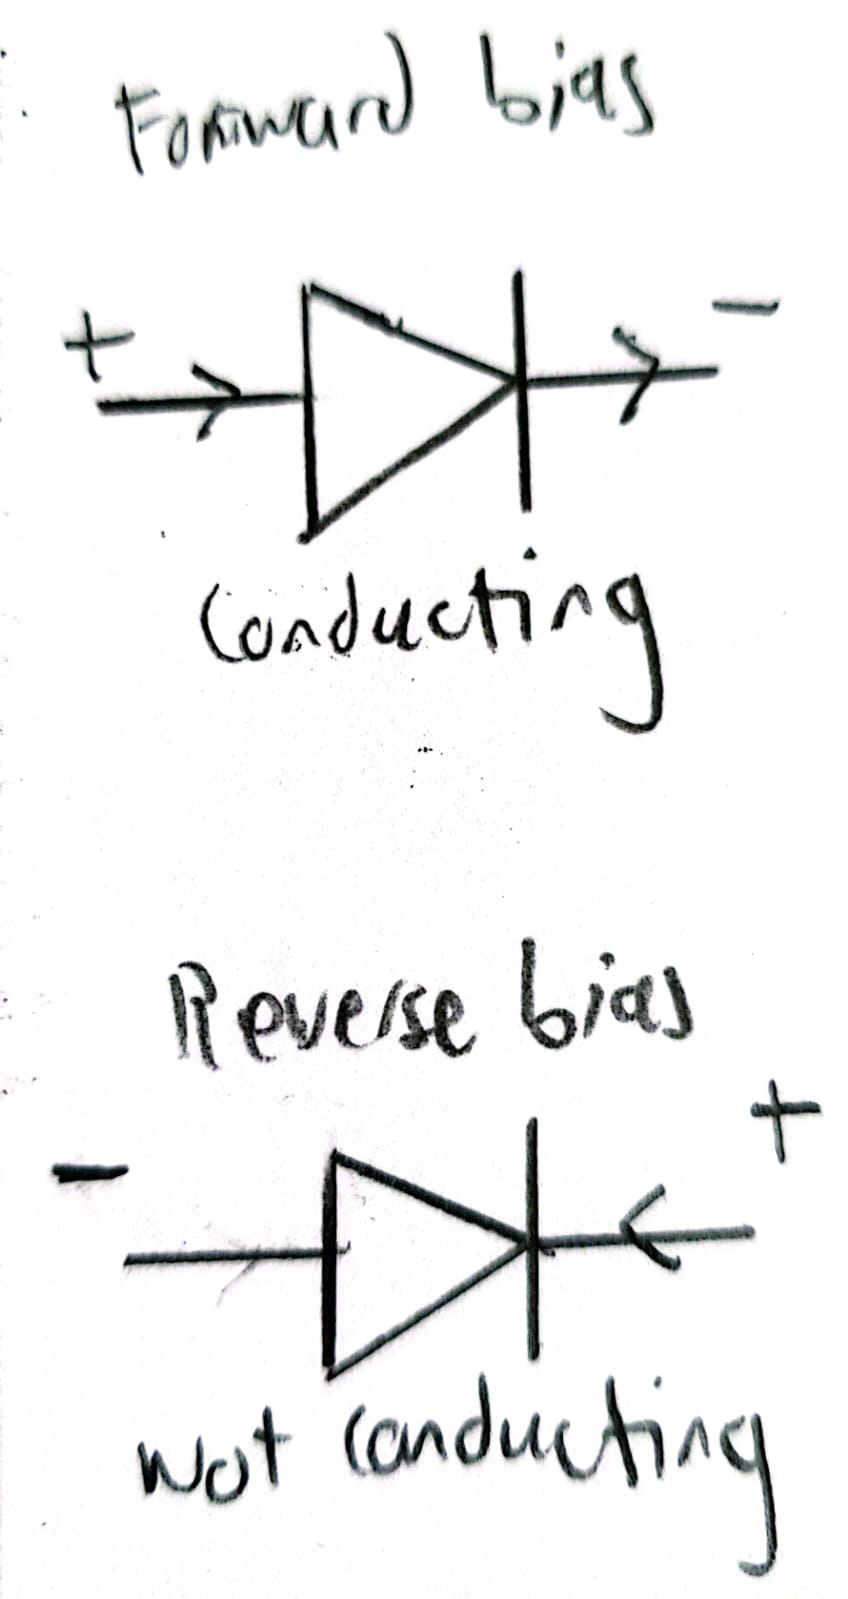
\includegraphics[scale=0.08]{../images/ForwardReverseBias.jpg}
            \end{center}
        \end{minipage} &
        \begin{minipage}{0.3\textwidth}
            \begin{itemize}
                    \item Forward-biased: \emph{Resistance decreases} when \emph{p.d. increases}. In fact, if the forward-biased p.d. goes past its \emph{threshold voltage}, \emph{resistance} becomes very low.
                    \item Reverse-biased: \emph{Very high resistance}. But, there will be a \emph{small leakage current}.
                    \item If the reverse-biased p.d. is so high that it exceeds the \emph{breakdown voltage}, the diode will \emph{break down} and \emph{conduct electricity}.
            \end{itemize} 
            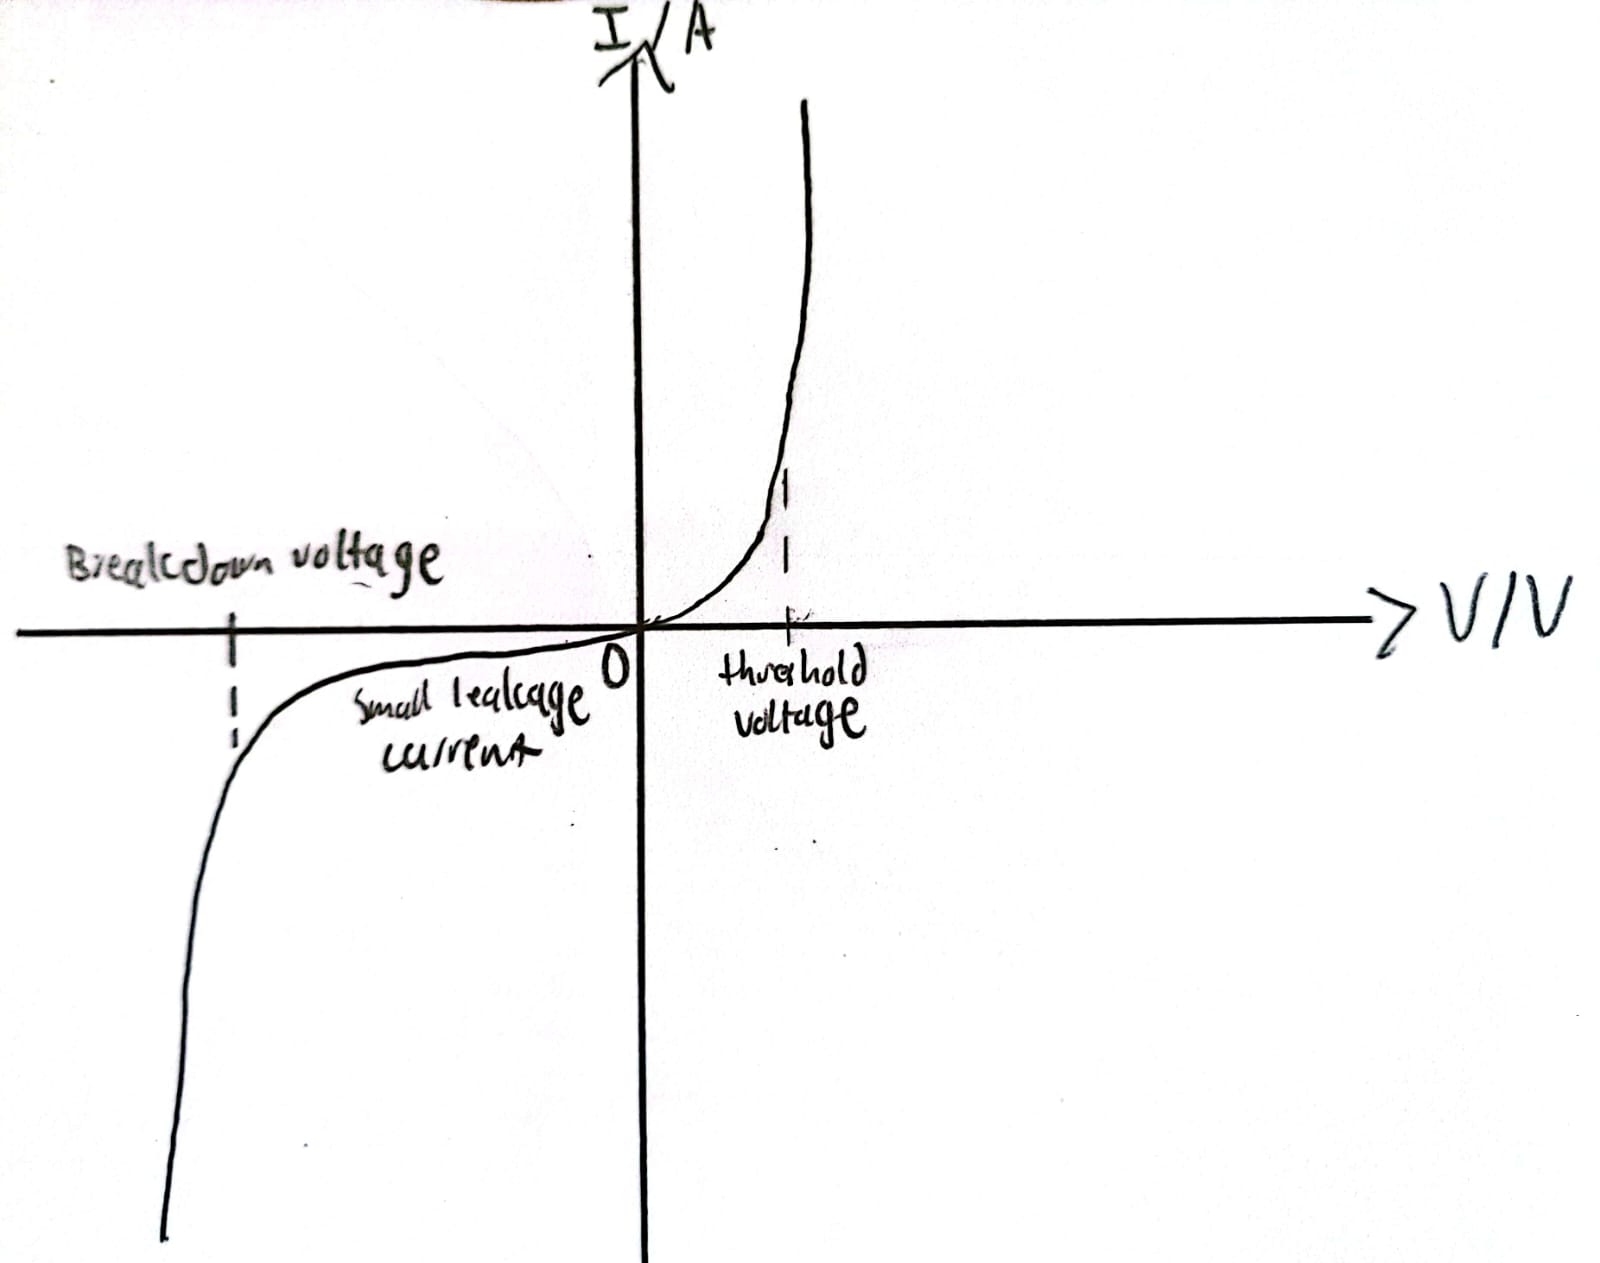
\includegraphics[width=\textwidth]{../images/Diode I-V characteristics.jpg}
        \end{minipage} &
        \begin{minipage}{0.3\textwidth}
            \begin{itemize}
                \item When connected in \emph{forward bias}, the circuit's \emph{electric field set up} allows for available \emph{charge carriers to flow} through, allowing it to conduct with \emph{low resistance}.
                \item When connected in \emph{reverse bias}, the circuit's electric field set up creates a \emph{widened `depletion region'} in the diode which \emph{impedes charge carriers} from flowing through the region, creating a \emph{large resistance}. 
            \end{itemize}
        \end{minipage}\\
        \hline
        \begin{minipage}{0.25\textwidth}
            Filament Lamp
        \end{minipage} &  
        \begin{minipage}{0.3\textwidth}
            \begin{itemize}
                \item When \emph{p.d. increases, current increases}, with \emph{decreasing \(I\)-\(V\) ratio}.
                \item The \emph{resistance} of a metallic conductor \emph{increases} with an increase in \emph{temperature}.
            \end{itemize} 
            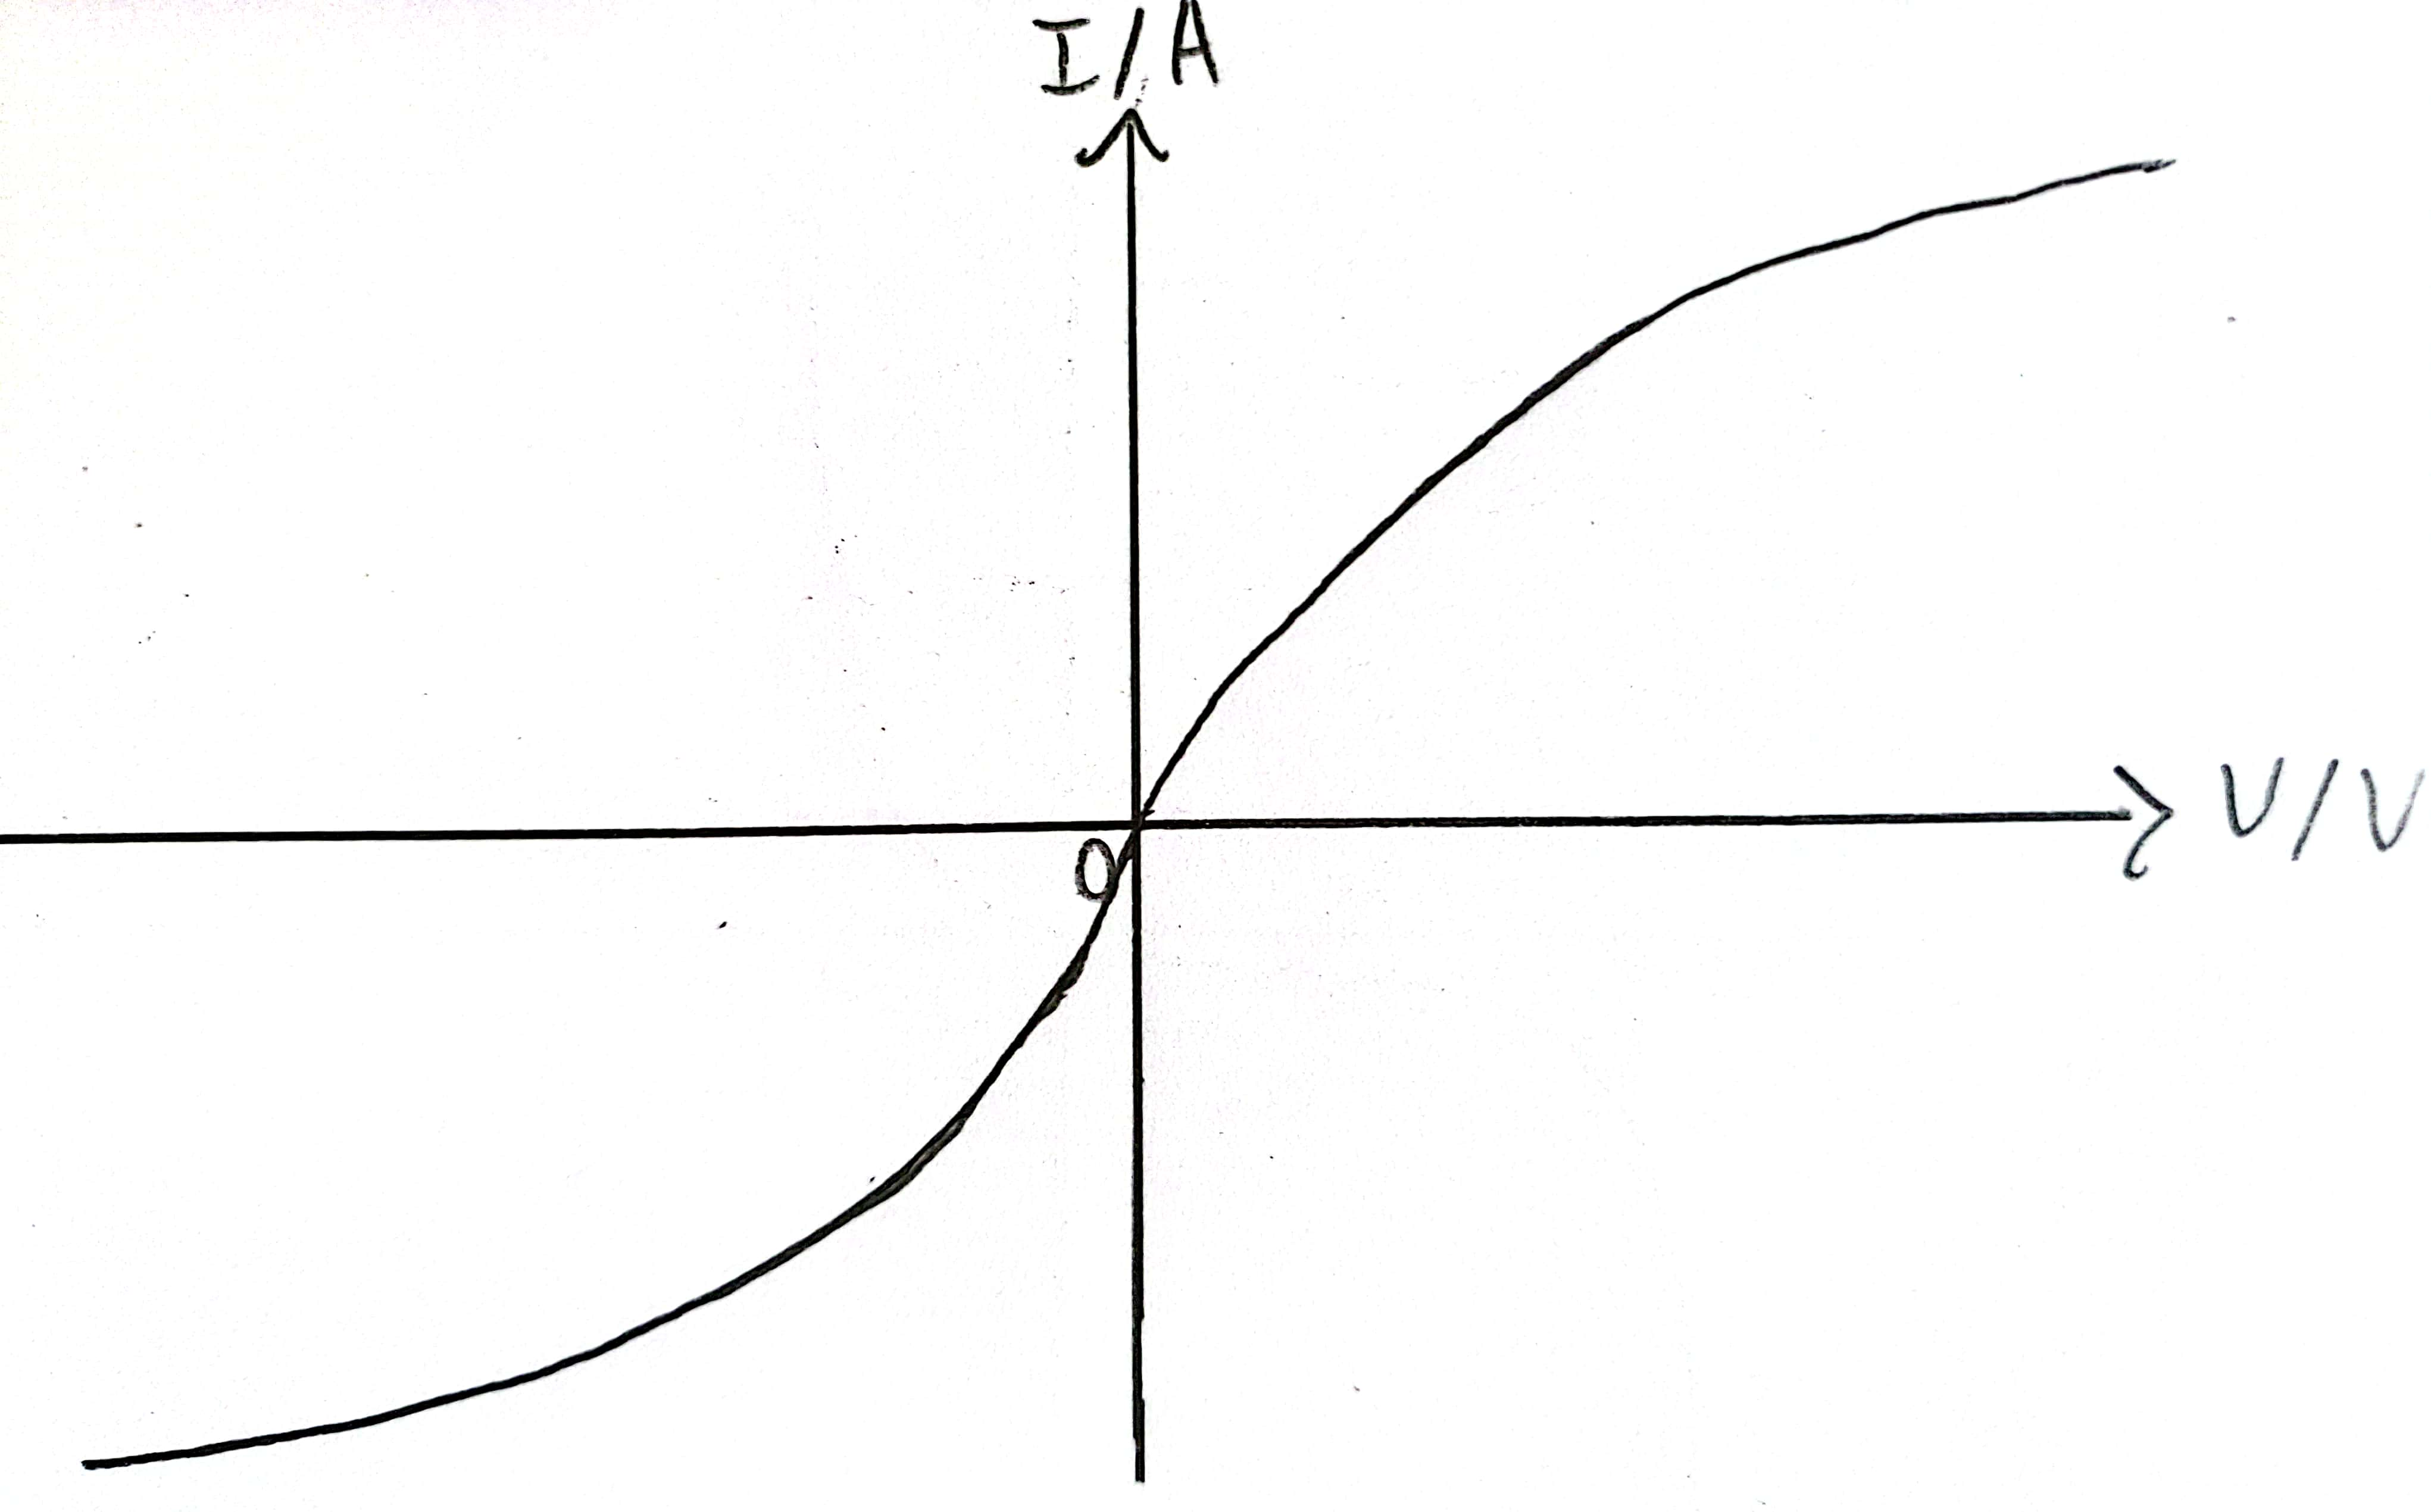
\includegraphics[width=\textwidth]{../images/Filament Lamp I-V Characteristics.jpg}\\[-1mm]
            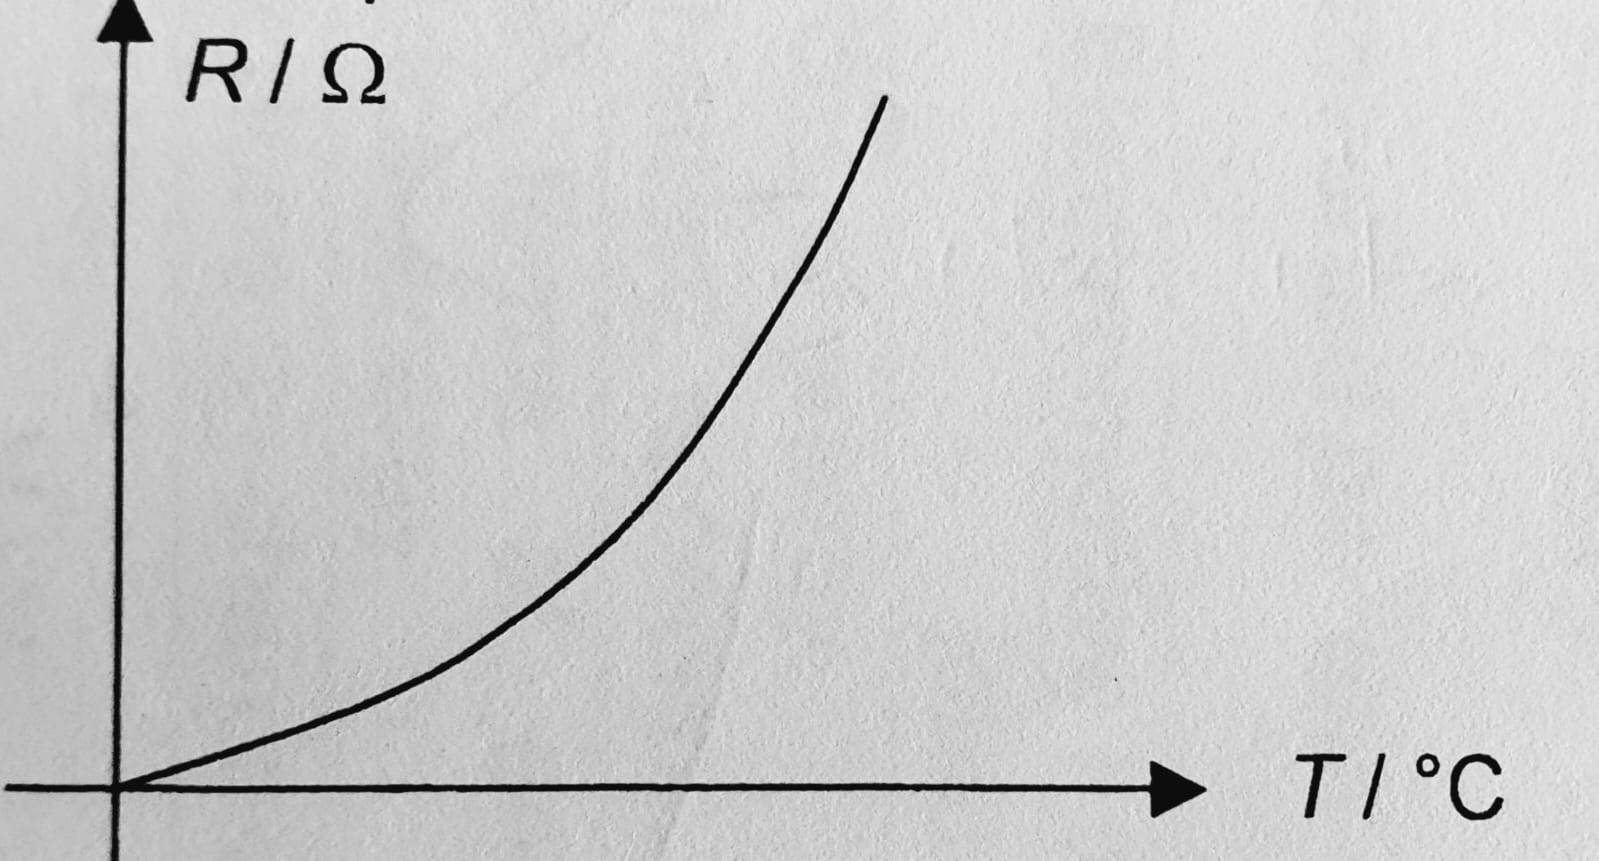
\includegraphics[width=\textwidth]{../images/Filament Lamp Resistance.jpg}
        \end{minipage} &
        \begin{minipage}{0.3\textwidth}
            \begin{itemize}
                \item As \emph{current increases, power dissipated increases} since \(P=I^2R\). Heat is generated so \emph{equilibrium temperature rises} --- as electrons drift through the metal, they collide with the metal lattice and transfers energy to it. 
                \item The \emph{lattice ions vibrate more vigorously}. This \emph{hinders the flow} of `charge carriers'. Therefore, \emph{resistance is increased}.
                \item Ohmic conductors hence do \emph{not} obey Ohm's Law at \emph{high} voltages/currents.
            \end{itemize}
        \end{minipage}\\
        \hline
        \begin{minipage}{0.25\textwidth}
            Negative Temperature Coefficient (NTC) Thermistor
        \end{minipage} &  
        \begin{minipage}{0.3\textwidth}
            \begin{itemize}
                \item When \emph{p.d. increases}, \emph{current} through the thermistor also \emph{increases}, with \emph{increasing \(I\)-\(V\) ratio}.
                \item The \emph{resistance} of a thermistor \emph{decreases} with an \emph{increase} in \emph{temperature} (This is the meaning of NTC).
            \end{itemize} 
            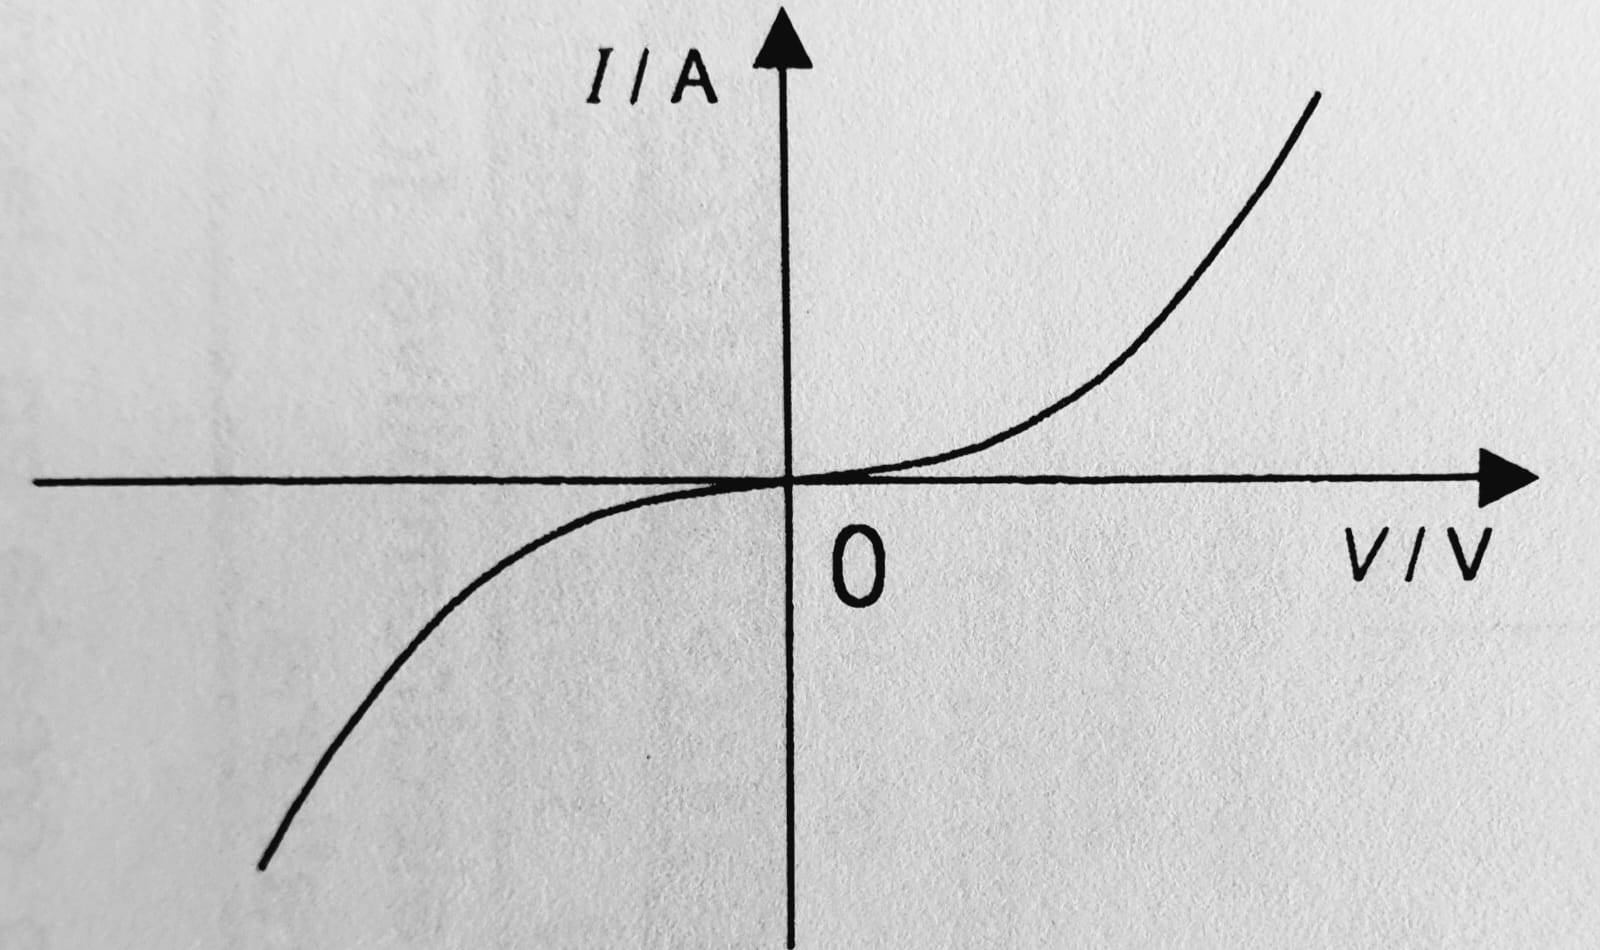
\includegraphics[width=\textwidth]{../images/NTC I-V.jpg}\\[-1mm]
            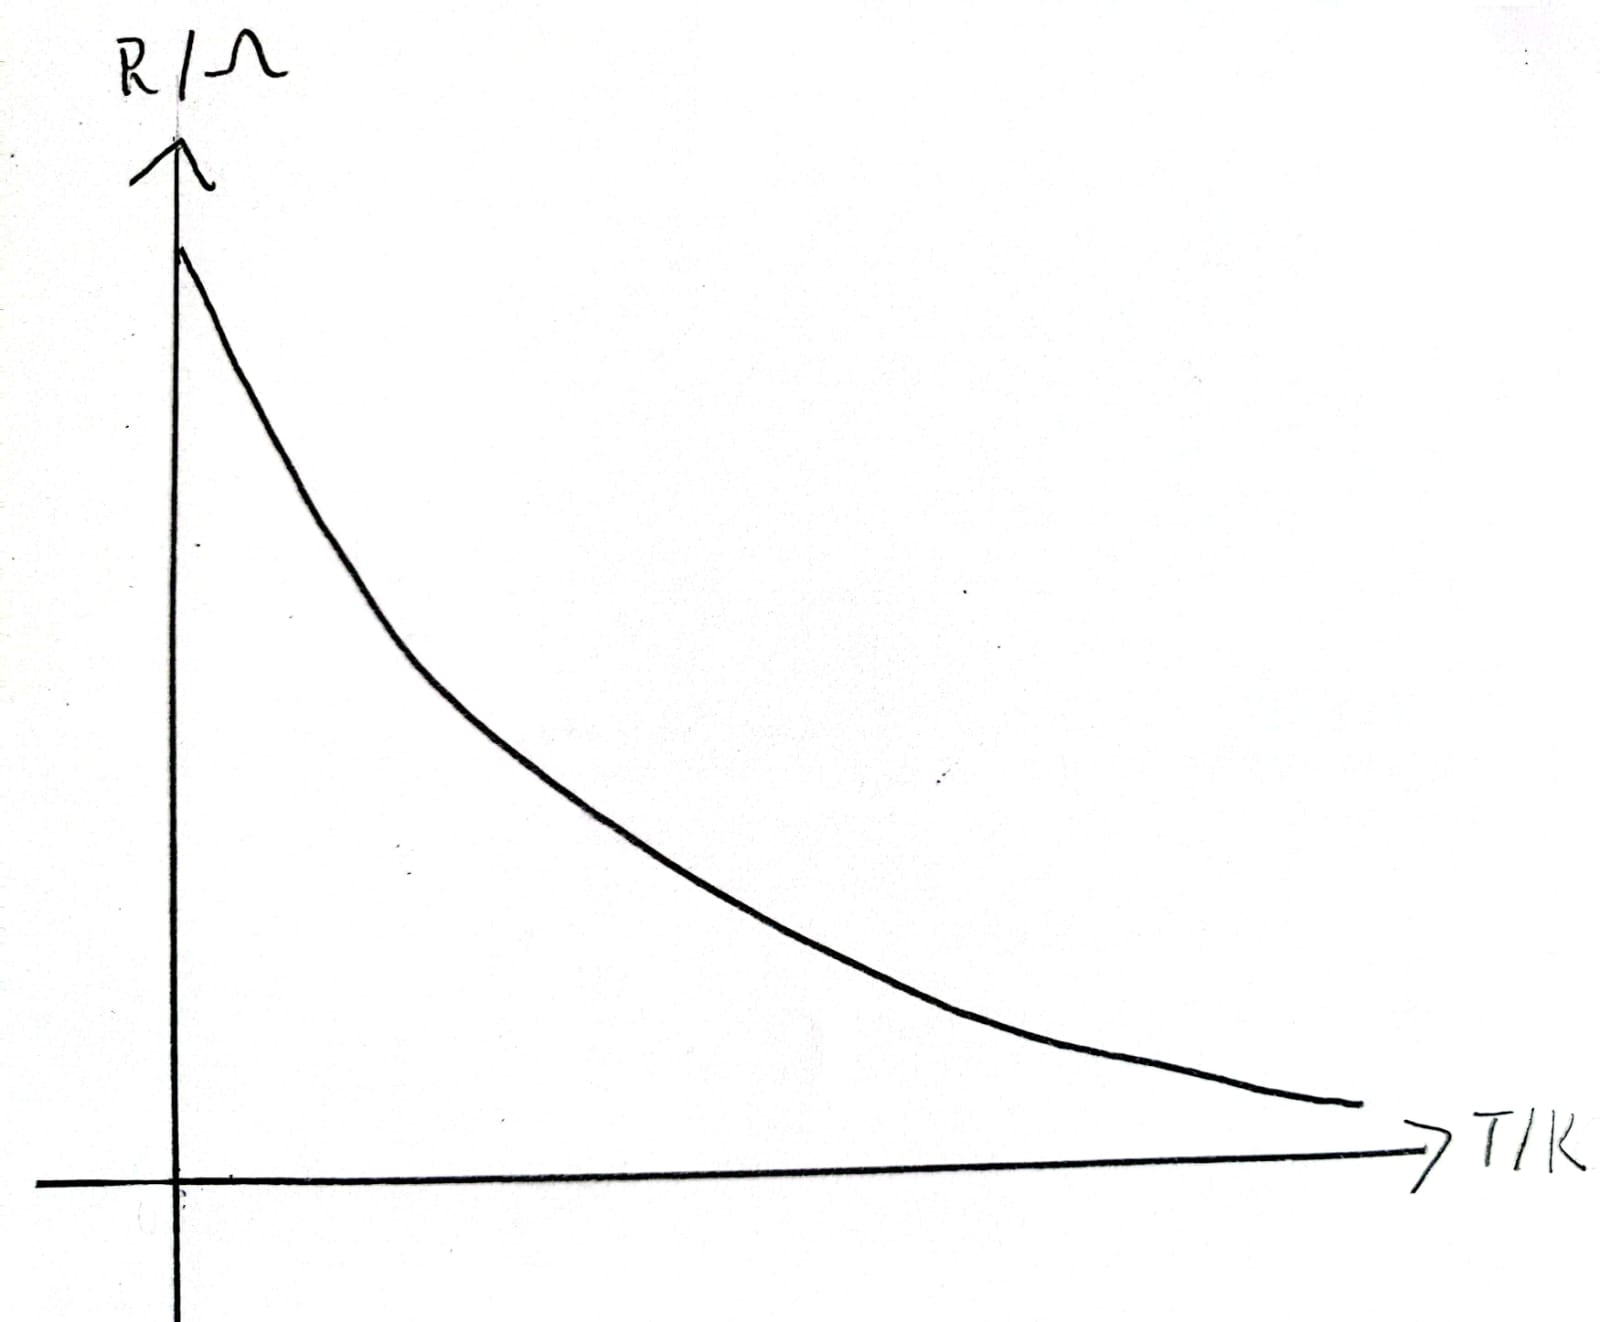
\includegraphics[width=\textwidth]{../images/NTC Resistance.jpg}
        \end{minipage} &
        \begin{minipage}{0.3\textwidth}
            \begin{itemize}
                \item  As \emph{current increases}, \emph{power dissipated increases}. \emph{More heat} is generated, leading to a \emph{rise} in \emph{equilibrium temperature}.
                \item Thus, the \emph{mean kinetic energy} of the electrons and lattice ions \emph{increases}. So,
            \end{itemize}
            \begin{enumerate}
                \item The \emph{bonded electrons break free} from bonds, increasing the \emph{number} of `mobile charge carriers'. Therefore, \emph{resistance decreases}.
                \item The \emph{lattice ions vibrate more vigorously}, \emph{hindering the flow} of `mobile charge carriers'. Thence, resistance increases.  
            \end{enumerate} 
            \begin{itemize}
                \item The first effect is much more significant than the second. So, there is a net \emph{decrease in resistance}.
            \end{itemize}
        \end{minipage}\\
        \hline
    \end{longtable}
    The images above come from \ref{Me}.
    \begin{example}{}{}
        Explain, in \emph{microscopic terms}, why the resistance of a wire increases as the current through it increases. \hspace*{\fill} [2]
        \begin{itemize}
            \item As current increases, the rate at which electrons collide into the metal lattice increases; temperature increases. \hspace*{\fill} [1]
            \item As temperature increases, lattice ions vibrate more vigorously, hindering the flow of electrons; resistance increases. \hspace*{\fill} [1]
        \end{itemize}
    \end{example}
    \item The \emph{electromotive force} (e.m.f) of a \emph{source} is defined as the amount of \emph{energy converted} from \emph{non-electrical} forms of energy to \emph{electrical} energy \emph{per unit charge} as the \emph{charge passes through a complete circuit}.
    \item Internal resistance: the p.d. across a component is given by \(V=E-Ir\).
    \item Power dissipated \(P=IV\).
    \item Power delivered is \emph{maximum } when \(R=r\), such that 
    \[P_{\text{max}}=\frac{E^2}{4r}.\]
    \emph{Note.} Unless specified by the question, try to avoid assuming that the internal resistance \(r\) of the internal resistance of a cell is constant, if possible.
    \item Efficiency of the source
    \begin{itemize}
        \item \emph{Increases} when external load/\emph{resistance increases}.
        \item Is halved when \(R=r\).

        \emph{Note:} Maximum power \(\neq\) maximum efficiency.
    \end{itemize}
\end{itemize}